% arara: lualatex: { shell : yes }
% arara: biber
% arara: lualatex: { shell : yes }
% arara: lualatex: { shell : yes }

% options:
% thesis=B bachelor's thesis
% thesis=M master's thesis
% czech thesis in Czech language
% slovak thesis in Slovak language
% english thesis in English language
% hidelinks remove colour boxes around hyperlinks

\documentclass[thesis=B,czech]{FITthesis}[2019/12/23]

\usepackage[utf8]{inputenc} % LaTeX source encoded as UTF-8

% \usepackage{amsmath} %advanced maths
% \usepackage{amssymb} %additional math symbols

\usepackage{dirtree} %directory tree visualisation

% % list of acronyms
% \usepackage[acronym,nonumberlist,toc,numberedsection=autolabel]{glossaries}
% \iflanguage{czech}{\renewcommand*{\acronymname}{Seznam pou{\v z}it{\' y}ch zkratek}}{}
% \makeglossaries

\usepackage[style=iso-numeric]{biblatex}
\addbibresource{mybibliographyfile.bib}

\usepackage{enumitem}

\usepackage{luavlna}

\usepackage{minted}
\counterwithin{listing}{chapter}
\renewcommand{\listingscaption}{Výpis kódu}
\renewcommand{\listoflistingscaption}{Seznam výpisů kódu}

\newcommand{\tg}{\mathop{\mathrm{tg}}} %cesky tangens
\newcommand{\cotg}{\mathop{\mathrm{cotg}}} %cesky cotangens

% % % % % % % % % % % % % % % % % % % % % % % % % % % % % % 
% ODTUD DAL VSE ZMENTE
% % % % % % % % % % % % % % % % % % % % % % % % % % % % % % 

\assignment{zadání}
\department{Katedra softwarového inženýrství}
\title{Editor zdrojových kódů WooWoo dokumentů}
\authorGN{David} %(křestní) jméno (jména) autora
\authorFN{Straka} %příjmení autora
\authorWithDegrees{David Straka} %jméno autora včetně současných akademických titulů
\author{David Straka} %jméno autora bez akademických titulů
\supervisor{Ing. Tomáš Kalvoda, Ph.D.}
\acknowledgements{\#todo Doplňte, máte-li komu a za co děkovat. V~opačném případě úplně odstraňte tento příkaz.}
\abstractCS{Tato práce se zabývá návrhem, implementací a otestováním rozšíření editoru Atom pro usnadnění tvorby WooWoo dokumentů.
Důraz je kladen zejména na přehlednou prezentaci logické struktury dokumentů využívajících existující šablony. Součástí
práce je také seznámení se s formátem WooWoo, rešerše možností rozšíření stávajících editorů nebo možností zobrazování
matematických výrazů a různých grafických objektů.
}
\abstractEN{This thesis deals with the design, implementation, and testing of an extension of the Atom editor for streamlining the
creation of WooWoo documents. Emphasis is put especially on clear presentation of the logical structure of documents
using the existing templates. Familiarization with the WooWoo format, research of the possibilities of the extension of
current editors and possibilities of displaying mathematical expressions and different graphic objects are all also part
of the thesis.
}
\placeForDeclarationOfAuthenticity{V~Praze}
\declarationOfAuthenticityOption{5} %volba Prohlášení (číslo 1-6)
\keywordsCS{WooWoo editor, Atom rozšíření, Atom package, WooWoo formát}
\keywordsEN{WooWoo editor, Atom extension, Atom package, WooWoo format}
\website{https://github.com/davidstraka2/bachelors-thesis} %volitelná URL práce, objeví se v tiráži - úplně odstraňte, nemáte-li URL práce

\begin{document}

% \newacronym{CVUT}{{\v C}VUT}{{\v C}esk{\' e} vysok{\' e} u{\v c}en{\' i} technick{\' e} v Praze}
% \newacronym{FIT}{FIT}{Fakulta informa{\v c}n{\' i}ch technologi{\' i}}

\begin{introduction}
	\input{content/úvod}
\end{introduction}

%\chapter{Cíl práce}

\chapter{Rešerše a analýza}
Pro realizaci rozšíření Atomu byl vybrán jazyk TypeScript. TypeScript je dle \cite{ts-docs} open-source nadstavba jazyka
JavaScript, která jej rozšiřuje o statickou typovou kontrolu. Díky kompilaci do jazyka JavaScript je pak výstup možné
použít v Atomu.

Kód rozšíření je doplněn o dokumentační komentáře. Dále byl využit nástroj Prettier pro formátování kódu a nástroj
ESLint pro statickou analýzu.

\section{Zvýrazňování syntaxe}
Podle \cite{atom-docs} v sobě Atom nabízí zabudované dva způsoby, jak přidat podporu zvýrazňování syntaxe pro nové
jazyky.

První, dle \cite{atom-docs} novější způsob je založený na nástroji Tree-sitter. Tree-sitter je dle \cite
{tree-sitter-docs} parser generátor, který na základě bezkontextové gramatiky zapsané v jeho vlastním formátu vygeneruje
parser, jehož výstupem je derivační strom (CST). Aby pak fungoval efektivně, mělo by dle \cite{tree-sitter-docs} navíc
jít o LR(1) gramatiku. Vygenerovaný parser je dle \cite{tree-sitter-docs} v jazyku C a lze ho pak použít i v jiných
aplikacích. Aby mohl být použit v Atomu, musí být dle \cite{atom-docs} zkompilován pro požadované platformy, spolu s tím
vygenerovány \textit{bindings} pro Node.js a tento celý výstup publikován jako knihovna na npm. Tuto knihovnu následně
dle \cite{atom-docs} využije vytvářený \textit{package} přidávající do Atomu podporu nového jazyka s pomocí \textit
{grammar} souboru v CSON nebo JSON formátu, ve kterém dále specifikuje, které vrcholy CST připadají kterému \textit
{grammar scope} (\textit{grammar scopes} v podstatě určují CSS třídu, která bude kódu, který odpovídá danému vrcholu,
přiřazena). Těmto \textit{grammar scopes} pak dle \cite{atom-docs} s pomocí odpovídajících CSS tříd přiřazují styly
různé další \textit{packages} přidávající do Atomu syntaktická témata.

Výhodou tohoto přístupu je, že podle \cite{atom-docs} funguje rychleji a přesněji (parser je založený na bezkontextové
gramatice namísto rozšířených regulárních výrazů), než dále zmíněná alternativa. Nevýhodou je, že i dle Tree-sitter
dokumentace \cite{tree-sitter-docs} je náročný na realizaci. Navíc vzhledem ke kontextově závislým prvkům WooWoo formátu
by takto vzniklý parser stejně nebyl schopen WooWoo parsovat zcela korektně a nemohl by tak být sám o sobě využit
například pro překlad do HTML pro náhled dokumentu.

Druhým způsobem je dle \cite{atom-docs} vytvoření gramatiky ve formátu založeném na TextMate gramatikách. Jedná se o
poměrně jednoduchý systém, který dle \cite{atom-docs} využívá (rozšířené) regulární výrazy. Postup vytvoření \textit
{grammar} souboru je zde dle \cite{atom-docs} podobný, jako v předchozím případě, pouze namísto vrcholů CST přiřazujeme
\textit{grammar scopes} vzorům popsaným (rozšířenými) regulárními výrazy (a samozřejmě zde odpadá definice použité
parser knihovny). Vnitřně pak dle \cite{atom-docs} Atom využívá engine (rozšířených) regulárních výrazů Oniguruma,
konkrétní podporované konstrukty v (rozšířených) regulárních výrazech jsou tedy dané právě tímto enginem.

Výhodou tohoto přístupu je jednoduchost implementace. Další výhodou je, že podobný způsob zvýrazňování syntaxe využívají
další populární editory (např. TextMate, po kterém je tento způsob zvýrazňování syntaxe pojmenovaný, dále třeba VS Code
\cite{vscode-docs} nebo Sublime Text \cite{sublime-text-docs}) a vytvořená gramatika by se tak dala s drobnými úpravami
použít i v nich. Nevýhodou tohoto přístupu je již zmiňovaná nižší rychlost a přesnost. Dále je nutno zmínit, že
Tree-sitter gramatiky jsou aktuálně dle \cite{atom-docs} preferovány a Atom na ně chce postupně přejít. Nicméně vzhledem
k velkému množství existujících TextMate gramatik není pravděpodobné, že by k nějakému úplnému ukončení jejich podpory
došlo v dohledné době.

Atom dále dle \cite{atom-docs} umožňuje namísto JSON/CSON souboru popsat gramatiku přímo v rámci API a dynamicky ji měnit
za běhu. Toho využivá například \textit{package} tasks \cite{atom-package-tasks}. V našem případě by toto mohlo být
užitečné například pro přesnější zvýrazňování syntaxe v závislosti na použité šabloně. Dále by tento přístup mohl
zmenšit opakování kódu (za předpokladu že by obdobné regulární výrazy byly využity také pro parsování) a lepší
testovatelnost.


\section{Parsování}
\#todo AST, parsování


\section{Zobrazení náhledu}
\begin{sloppypar}
Náhled dokumentu je realizován v samostatném podoknu Atomu, které si uživatel může v pracovním prostředí Atomu zobrazit
s pomocí příkazu \mintinline{text}{wootom:togglePreview}, klávesové zkratky (ve výchozím nastavení \textsc{Alt~+~J}),
položky \uv{Wootom: Toggle Preview} v kontextovém menu nebo podpoložky \uv{Toggle Preview} položky \uv{Wootom} v hlavním
menu Atomu.
\end{sloppypar}

Po zobrazení podokna náhledu (nejprve se otevře napravo podokna editoru aktuálně otevřeného souboru, uživatel se poté
může podokno přemístit) je aktuálně otevřený soubor rozparsován do AST.

\begin{sloppypar}
Poté co je dokument rozparsován, je vzniklý AST reprezentující obsah WooWoo dokumentu podán metodě
\mintinline{text}{RenderingManager#render}. Tato metoda přijme kořen AST, získá pro něj příslušnou implementaci
\mintinline{text}{Renderer} (viz výpis kódu \ref{zobrazeni-nahledu-renderer}) z registru
\mintinline{text}{RendererRegistry}, zavolá metodu \mintinline{text}{Renderer#render} na tento kořen a její výsledek
vrátí. Metoda \mintinline{text}{Renderer#render} pak může teoreticky s přijmutým vrcholem dělat cokoliv, ale v typickém
případě vrchol stromu nějakým způsobem tranformuje na HTML, na všechny jeho děti opět zavolá
\mintinline{text}{RenderingManager#render} a výsledky (HTML vrcholy) těchto volání přidá jako obsah do svého HTML. Takto
se renderování postupně zanořuje hlouběji a hlouběji až projde celý AST. Pokud je navíc některý z vrcholů, které
\mintinline{text}{RenderingManager#render} zpracovává, jedním z druhů prvků WooWoo dokumentu, které mají variantu,
před hledáním příslušného \mintinline{text}{Renderer} v \mintinline{text}{RendererRegistry} je navíc získána abstraktní
varianta z \mintinline{text}{VariantRegistry}. Pokud abstraktní varianta nebyla nalezena, je použit výchozí
\mintinline{text}{Renderer}.
\end{sloppypar}

\begin{sloppypar}
Takto je z AST získáno HTML reprezentující logickou strukturu WooWoo dokumentu. Toto HTML je následně podáno metodě
\mintinline{text}{HTMLViewModel#render}, která jej zobrazí uživateli v podoknu pro náhled.
\end{sloppypar}

\begin{listing}
    \caption{Interface \mintinline{typescript}{Renderer}}
    \label{zobrazeni-nahledu-renderer}
    \begin{minted}{typescript}
interface Renderer {
    kind?: WooElementKind;
    abstractVariant?: string;

    render<T extends ASTNode>(
        renderingManager: RenderingManager,
        astNode: T,
    ): Node;
}
    \end{minted}
\end{listing}

Na obrázku \ref{zobrazeni-nahledu-pkm-kapitola} je pro ilustraci zobrazen náhled dokumentu s definicí části (zde
konkrétně kapitoly), jejím meta-blokem a následujícím blokem textu (zdroj dokumentu vzatý ze studijního textu BI-PKM).

\begin{figure}\centering
    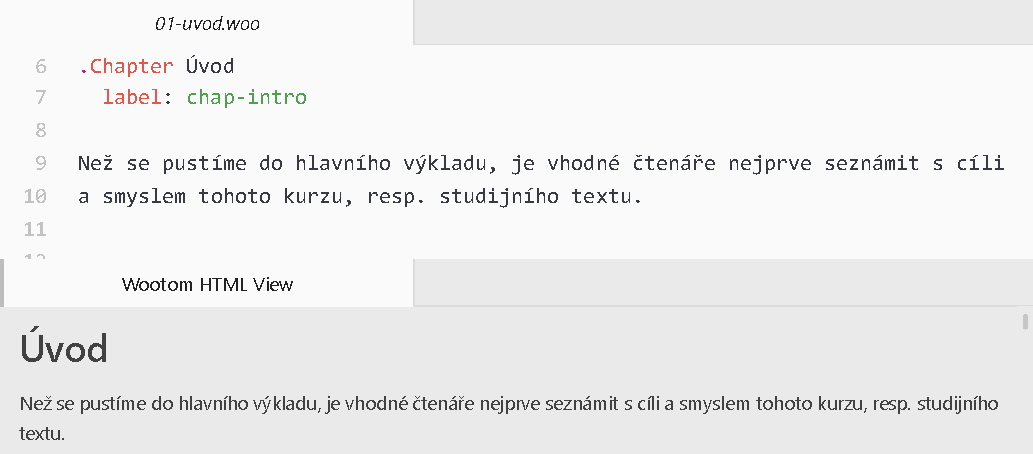
\includegraphics[width=1.0\textwidth]{content/realizace/zobrazení-náhledu-pkm-kapitola}
 	\caption[Náhled části dokumentu]{Náhled části dokumentu ve zdroji studijního textu k BI-PKM~\cite{pkm}}
    \label{zobrazeni-nahledu-pkm-kapitola}
\end{figure}

\begin{sloppypar}
Náhled je živě aktualizován při modifikaci zdrojového souboru. Bylo implementováno jednoduché zobrazování většiny prvků
FIT Template šablony dle stylů existujících výstupů. Zobrazování některých prvků ale zatím podporováno není. Z časových
důvodů nebylo implementováno zobrazení vnějších prostředí \mintinline{text}{.enumerate} a \mintinline{text}{.itemize}
a vnitřního prostředí \mintinline{text}{.item}. Dále nebylo implementováno zobrazování vnějšího prostředí \mintinline
{text}{.image} a vnitřního prostředí \mintinline{text}{.todo}, a to z důvodu jejich absence ve zdrojích existujících
studijních textů. Všechny ostatní prvky jsou (alespoň částečně) zobrazovány.
\end{sloppypar}

Tímto je realizován funkční požadavek \textbf{\ref{F2}} a \textbf{\ref{F3}}. V budoucnu by mohl být náhled vylepšen
například o zobrazení celého dokumentu (nikoliv pouze aktuálně otevřeného souboru) nebo o synchronní posuv náhledu a
zdrojového souboru (což by mělo být možné díky přesným pozicím vrcholů AST).

\subsection{Zobrazování matematických výrazů}

Zobrazování matematických výrazů je na základě provedené rešerše \ref{zobrazovani-matematickych-vyrazu} řešeno za pomoci
knihovny MathJax 2.x s konfigurací SVG výstupu. Uživateli je dále umožněno nadefinovat v nastaveních rozšíření vlastní
makra, která jsou předána konfiguraci knihovny MathJax.

Na obrázku \ref{zobrazeni-nahledu-pkm-matematika} je pro ukázku zobrazen náhled vnitřních matematických prostředí v textu,
jež jsou doplněna o vnější matematické prostředí (blokovou matematiku).

\begin{figure}\centering
    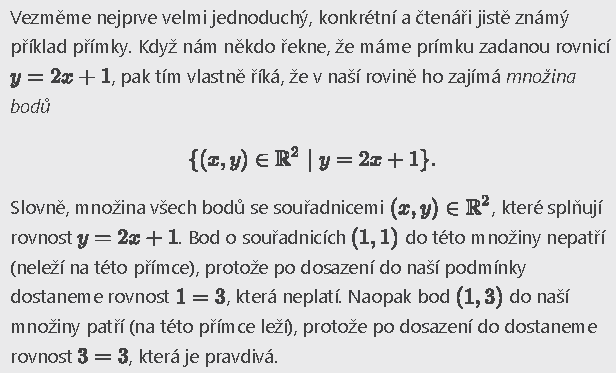
\includegraphics[width=1.0\textwidth]{content/realizace/zobrazení-náhledu-pkm-matematika}
 	\caption[Matematické výrazy v náhledu dokumentu]{Matematické výrazy v náhledu studijního textu k BI-PKM~\cite{pkm}}
    \label{zobrazeni-nahledu-pkm-matematika}
\end{figure}

Protože je sazba matematických výrazů výpočetně náročná, jsou výstupní SVG jsou cachována v paměti (do zavření editoru)
a je-li stejný výraz použit znovu (při obnovení náhledu nebo třeba v jiném souboru), MathJax už volán není a výsledné
SVG je zobrazeno mnohem rychleji (zdánlivě okamžitě).

Byl tak realizován funkční požadavek \textbf{\ref{F4}}.

\subsection{Zobrazování grafických objektů}

Zobrazování TikZ obrázků je na základě provedené rešerše \ref{zobrazovani-grafickych-objektu} řešeno závislostí na
nativní instalaci \TeX{} distribuce. Obdobně jako uživatel může v nastaveních nadefinovat vlastní makra pro MathJax, tak
i zde je umožněno do preambule \LaTeX{} dokumentu, který je použit pro vygenerování obrázku, vložit vlastní obsah (nejen
vlastní makra, ale například i použití dalších \LaTeX{} \textit{packages}).

Při překladu vrcholu AST, který reprezentuje vnější prostředí \mintinline{text}{!tikz}, je nejprve zobrazeno HTML se
(částečně skrytým) zdrojem TikZ. Při tomto překladu je zároveň zavolána asynchronní funkce, která nejprve zkontroluje,
zdali se zdroj obrázku nenachází v cache. Pokud ano, je vrácen obsah cache (kterým je výsledné SVG) a ten je zobrazen
uživateli. Pokud ne, je TikZ zdroj spolu s preambulí (výchozí, nebo uživatelem definovanou) zapsán do dočasného souboru,
na který je zavolán příkaz \mintinline{text}{latex}, jehož výsledkem je DVI soubor (jehož generování je rychlejší, než
PDF). Pro vygenerování SVG z DVI je pak využit příkaz \mintinline{text}{dvisvgm}. Nakonec je SVG výstup přečten, přidán
do cache, jsou uklizeny dočasné soubory a obrázek je zobrazen uživateli. Pokud při procesu nastala chyba, je uživateli
zobrazen namísto obrázku obsah \LaTeX{} logu (log soubor je pak také odstraněn). Cache funguje stejným způsobem jako
cache pro MathJax výstup (je pouze v paměti, po zavření editoru je ztracena).

Protože vygenerované SVG má fixní barvy výplně, je pro podporu různých témat uživatelského rozhraní uživateli umožněno
vybrat v nastaveních jeden ze tří režimů zobrazování těchto SVG výstupů. Výchozím režimem je zobrazení obrázků s bílým
pozadím, dalším režimem pak inverze barev SVG a posledním režimem je zobrazení SVG bez jakýchkoliv změn (není přidáno
pozadí ani pozměněny barvy).

Tímto byl realizován funkční požadavek \textbf{\ref{F5}}. Ukázka náhledu TikZ obrázku se nachází na obrázku \ref
{zobrazeni-nahledu-pkm-tikz}.

\begin{figure}\centering
    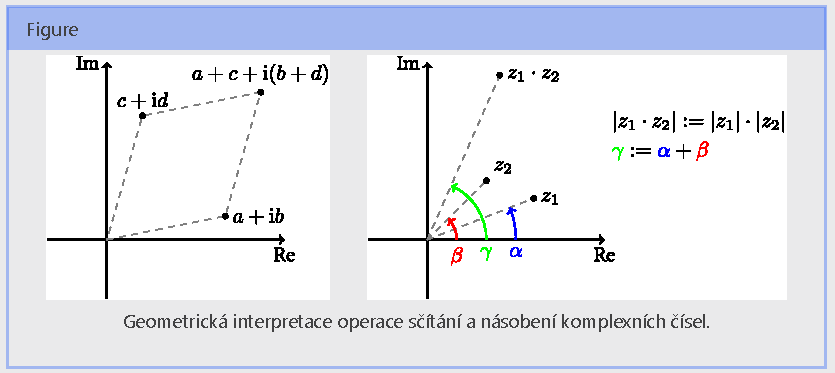
\includegraphics[width=1.0\textwidth]{content/realizace/zobrazení-náhledu-pkm-tikz}
 	\caption[TikZ obrázky v náhledu dokumentu]{TikZ obrázky v náhledu studijního textu k BI-PKM~\cite{pkm}}
    \label{zobrazeni-nahledu-pkm-tikz}
\end{figure}


\section{Navigace}
Navigace v dokumentu je realizována v podobě navigačního podokna, které si uživatel může v pracovním prostředí Atomu
zobrazit s pomocí příkazu \mintinline{text}{wootom:toggleNavigation}, klávesové zkratky (ve výchozím nastavení \textit
{Alt + N}), položky \uv{Wootom: Toggle Navigation} v kontextovém menu nebo podpoložky \uv{Toggle Navigation} položky
\uv{Wootom} v hlavním menu Atomu.

\begin{sloppypar}
Po zobrazení navigačního podokna (které se nejprve zobrazí napravo podokna editoru aktuálně otevřeného souboru; uživatel
si jej případně může přemístit) je aktuálně otevřený soubor rozparsován do AST. Z AST je pak získán seznam všech vrcholů,
které reprezentují části dokumentu a seznam všech vrcholů, které mají v meta-datech neprázdnou položku \mintinline{text}
{label}.
\end{sloppypar}

Ze seznamu vrcholů částí dokumentu je pak vytvořena jednoduchá stromová struktura reflektující úrovně konkrétních částí
(toto je potřeba provést, protože vytvořený AST části nevnořuje podle úrovně) z té je vytvořen číslovaný víceúrovňový
HTML seznam obsahující nadpisy daných částí. Nadpisy jsou přeloženy do HTML s pomocí volání \mintinline{text}
{RenderingManager#render}, čímž je zajištěno i zobrazení případných vnitřních prostředí. Seznam vrcholů AST se značkou
je abecedně seřazen a poté je z něj vytvořen jednoduchý nečíslovaný HTML seznam, obsahující název značky, druh vrcholu
(případě také jeho variantu) a jeho počáteční řádek. Všem položkám obou HTML seznamů je přidán \textit{event listener}
pro událost \textit{click}, který při kliknutí na položku seznamu skočí v editoru aktuálně otevřeného souboru na pozici
začátku daného prvku.

Tyto HTML seznamy jsou vloženy do navigačního podokna a pro přehlednost uvedeny nadpisy. Mezi nadpis a seznam je pak
vždy vloženo textové pole, s jehož pomocí může uživatel v seznamu vyhledávat relevantní položky. Vyhledávání je spuštěno
při libovolném uživatelském vstupu; pokud uživatel svůj dotaz vymaže, je vyhledávání zrušeno. Při vyhledávání v seznamu
částí dokumentu je vyhledáváno v textech nadpisů částí a výsledný seznam je zploštěn (už není víceúrovňový). Při
vyhledávání v seznamu značek je vyhledáváno pouze v názvech značek. Seznam výsledků vyhledávání je seřazen od největší
shody po nejnižší shodu.

Pro vyhledávání byla využita knihovna Fuse.js, která umožňuje fuzzy vyhledávání, kdy dotaz uživatele nemusí přesně
odpovídat vyhledávanému textu (dle dokumentace \cite{fuse-docs} knihovna využívá modifikovanou verzi algoritmu Bitap).
Tato knihovna byla dále vybrána díky její přehledné dokumentaci, dostupnosti TypeScript \textit{types}, permisivní
open-source licenci a velké popularitě (mezi 1,5 miliony a 3 miliony týdenních stažení z npm \cite{npm} za poslední
rok). Knihovna dále dle \cite{fuse-docs} umožňuje upravit mnoho různých parametrů vyhledávání, takže je v případném
budoucím vývoji možno například upravit mezi, které musí shoda dotazu a vyhledávaného textu dosáhnout.

Na obrázku \ref{navigace-pkm} je pro ilustraci zobrazeno okno Atomu s otevřeným souborem zdroje studijního textu k
BI-PKM na levé straně a jeho navigačním podoknem na pravé straně.

\begin{figure}\centering
    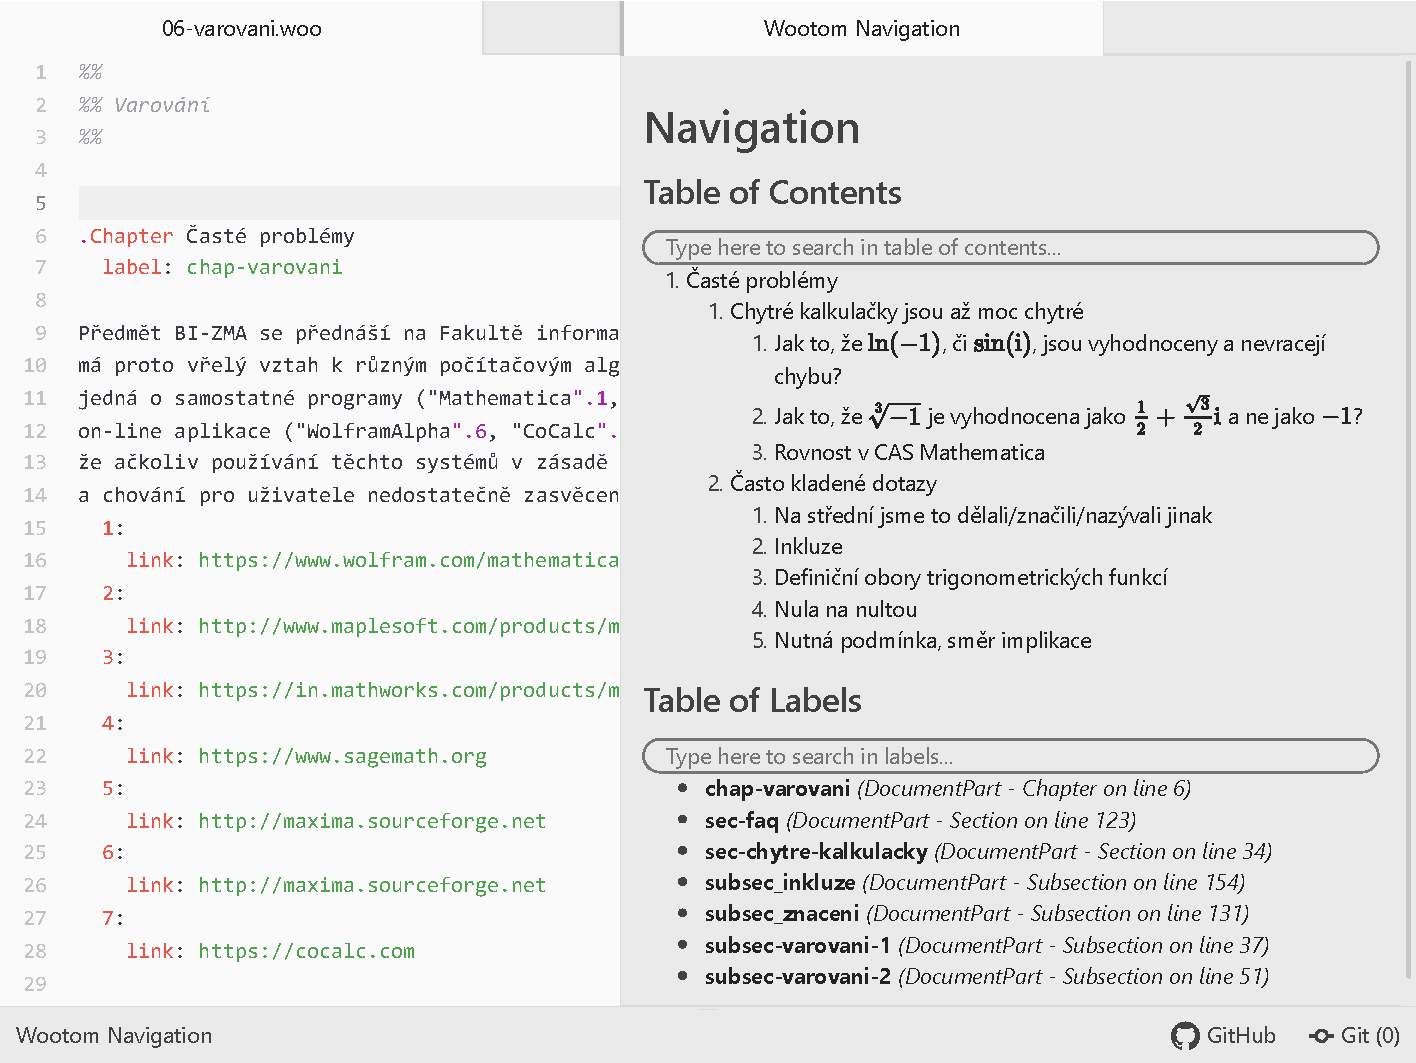
\includegraphics[width=1.0\textwidth]{content/realizace/navigace-pkm}
 	\caption[Navigace v dokumentu]{Navigační podokno u otevřeného souboru zdroje studijního textu k BI-PKM \cite{pkm}}
    \label{navigace-pkm}
\end{figure}

Tímto byly realizovány funkční požadavky \textbf{F6} až \textbf{F10}. Implementaci by bylo dále možno vylepšit například
o zobrazení přehledu částí a značek v celém dokumentu (nikoliv v pouze aktuálně otevřeném souboru).


\section{Testování}
Atom poskytuje v sobě zabudovaný systém pro spouštění testů, takzvaný test runner, postavený na testovacím frameworku
Jasmine. Všechny testy musí být ve složce \mintinline{text}{spec} v kořenové složce package a musí mít ve jméně příponu
\mintinline{text}{-spec} (tedy například \mintinline{text}{main-spec.js}). Následně je všechny testy možno spustit z
terminálu příkazem \mintinline{shell}{atom --test spec} (případně lze namísto celé složky s testy použít seznam
konkrétních souborů s testy), nebo přímo z Atomu s pomocí příkazu \mintinline{text}{window:run-package-specs}, za
předpokladu, že je jako aktuální projekt otevřen testovaný package. \cite{atom-man-specs}

Tento Atomem poskytovaný test runner nicméně vnitřně využívá Jasmine ve verzi 1.3. \cite{atom-man-specs} Jedná se o
poněkud starší verzi z roku 2013. \cite{jasmine-old-release} Chceme-li použít novější verzi Jasmine, nebo dokonce úplně
jiný testovací framework, můžeme využít možnosti vytvoření vlastního test runner. Takto vytvořené test runners pak jde
navíc jednoduše poskytnout ostatním pro využití v jejich packages, které si test runner pouze stáhnou jako závislost z
npm a v \mintinline{text}{package.json} řeknou Atomu, že chtějí využít onen konkrétní test runner. \cite{atom-man-specs}

\#todo Výběr konkrétního test runneru



\chapter{Realizace}
Pro realizaci rozšíření Atomu byl vybrán jazyk TypeScript. TypeScript je dle \cite{ts-docs} open-source nadstavba jazyka
JavaScript, která jej rozšiřuje o statickou typovou kontrolu. Díky kompilaci do jazyka JavaScript je pak výstup možné
použít v Atomu.

Kód rozšíření je doplněn o dokumentační komentáře. Dále byl využit nástroj Prettier pro formátování kódu a nástroj
ESLint pro statickou analýzu.

\section{Zvýrazňování syntaxe}
Podle \cite{atom-docs} v sobě Atom nabízí zabudované dva způsoby, jak přidat podporu zvýrazňování syntaxe pro nové
jazyky.

První, dle \cite{atom-docs} novější způsob je založený na nástroji Tree-sitter. Tree-sitter je dle \cite
{tree-sitter-docs} parser generátor, který na základě bezkontextové gramatiky zapsané v jeho vlastním formátu vygeneruje
parser, jehož výstupem je derivační strom (CST). Aby pak fungoval efektivně, mělo by dle \cite{tree-sitter-docs} navíc
jít o LR(1) gramatiku. Vygenerovaný parser je dle \cite{tree-sitter-docs} v jazyku C a lze ho pak použít i v jiných
aplikacích. Aby mohl být použit v Atomu, musí být dle \cite{atom-docs} zkompilován pro požadované platformy, spolu s tím
vygenerovány \textit{bindings} pro Node.js a tento celý výstup publikován jako knihovna na npm. Tuto knihovnu následně
dle \cite{atom-docs} využije vytvářený \textit{package} přidávající do Atomu podporu nového jazyka s pomocí \textit
{grammar} souboru v CSON nebo JSON formátu, ve kterém dále specifikuje, které vrcholy CST připadají kterému \textit
{grammar scope} (\textit{grammar scopes} v podstatě určují CSS třídu, která bude kódu, který odpovídá danému vrcholu,
přiřazena). Těmto \textit{grammar scopes} pak dle \cite{atom-docs} s pomocí odpovídajících CSS tříd přiřazují styly
různé další \textit{packages} přidávající do Atomu syntaktická témata.

Výhodou tohoto přístupu je, že podle \cite{atom-docs} funguje rychleji a přesněji (parser je založený na bezkontextové
gramatice namísto rozšířených regulárních výrazů), než dále zmíněná alternativa. Nevýhodou je, že i dle Tree-sitter
dokumentace \cite{tree-sitter-docs} je náročný na realizaci. Navíc vzhledem ke kontextově závislým prvkům WooWoo formátu
by takto vzniklý parser stejně nebyl schopen WooWoo parsovat zcela korektně a nemohl by tak být sám o sobě využit
například pro překlad do HTML pro náhled dokumentu.

Druhým způsobem je dle \cite{atom-docs} vytvoření gramatiky ve formátu založeném na TextMate gramatikách. Jedná se o
poměrně jednoduchý systém, který dle \cite{atom-docs} využívá (rozšířené) regulární výrazy. Postup vytvoření \textit
{grammar} souboru je zde dle \cite{atom-docs} podobný, jako v předchozím případě, pouze namísto vrcholů CST přiřazujeme
\textit{grammar scopes} vzorům popsaným (rozšířenými) regulárními výrazy (a samozřejmě zde odpadá definice použité
parser knihovny). Vnitřně pak dle \cite{atom-docs} Atom využívá engine (rozšířených) regulárních výrazů Oniguruma,
konkrétní podporované konstrukty v (rozšířených) regulárních výrazech jsou tedy dané právě tímto enginem.

Výhodou tohoto přístupu je jednoduchost implementace. Další výhodou je, že podobný způsob zvýrazňování syntaxe využívají
další populární editory (např. TextMate, po kterém je tento způsob zvýrazňování syntaxe pojmenovaný, dále třeba VS Code
\cite{vscode-docs} nebo Sublime Text \cite{sublime-text-docs}) a vytvořená gramatika by se tak dala s drobnými úpravami
použít i v nich. Nevýhodou tohoto přístupu je již zmiňovaná nižší rychlost a přesnost. Dále je nutno zmínit, že
Tree-sitter gramatiky jsou aktuálně dle \cite{atom-docs} preferovány a Atom na ně chce postupně přejít. Nicméně vzhledem
k velkému množství existujících TextMate gramatik není pravděpodobné, že by k nějakému úplnému ukončení jejich podpory
došlo v dohledné době.

Atom dále dle \cite{atom-docs} umožňuje namísto JSON/CSON souboru popsat gramatiku přímo v rámci API a dynamicky ji měnit
za běhu. Toho využivá například \textit{package} tasks \cite{atom-package-tasks}. V našem případě by toto mohlo být
užitečné například pro přesnější zvýrazňování syntaxe v závislosti na použité šabloně. Dále by tento přístup mohl
zmenšit opakování kódu (za předpokladu že by obdobné regulární výrazy byly využity také pro parsování) a lepší
testovatelnost.


\section{Parsování}
\#todo AST, parsování


\section{Zobrazení náhledu}
\begin{sloppypar}
Náhled dokumentu je realizován v samostatném podoknu Atomu, které si uživatel může v pracovním prostředí Atomu zobrazit
s pomocí příkazu \mintinline{text}{wootom:togglePreview}, klávesové zkratky (ve výchozím nastavení \textsc{Alt~+~J}),
položky \uv{Wootom: Toggle Preview} v kontextovém menu nebo podpoložky \uv{Toggle Preview} položky \uv{Wootom} v hlavním
menu Atomu.
\end{sloppypar}

Po zobrazení podokna náhledu (nejprve se otevře napravo podokna editoru aktuálně otevřeného souboru, uživatel se poté
může podokno přemístit) je aktuálně otevřený soubor rozparsován do AST.

\begin{sloppypar}
Poté co je dokument rozparsován, je vzniklý AST reprezentující obsah WooWoo dokumentu podán metodě
\mintinline{text}{RenderingManager#render}. Tato metoda přijme kořen AST, získá pro něj příslušnou implementaci
\mintinline{text}{Renderer} (viz výpis kódu \ref{zobrazeni-nahledu-renderer}) z registru
\mintinline{text}{RendererRegistry}, zavolá metodu \mintinline{text}{Renderer#render} na tento kořen a její výsledek
vrátí. Metoda \mintinline{text}{Renderer#render} pak může teoreticky s přijmutým vrcholem dělat cokoliv, ale v typickém
případě vrchol stromu nějakým způsobem tranformuje na HTML, na všechny jeho děti opět zavolá
\mintinline{text}{RenderingManager#render} a výsledky (HTML vrcholy) těchto volání přidá jako obsah do svého HTML. Takto
se renderování postupně zanořuje hlouběji a hlouběji až projde celý AST. Pokud je navíc některý z vrcholů, které
\mintinline{text}{RenderingManager#render} zpracovává, jedním z druhů prvků WooWoo dokumentu, které mají variantu,
před hledáním příslušného \mintinline{text}{Renderer} v \mintinline{text}{RendererRegistry} je navíc získána abstraktní
varianta z \mintinline{text}{VariantRegistry}. Pokud abstraktní varianta nebyla nalezena, je použit výchozí
\mintinline{text}{Renderer}.
\end{sloppypar}

\begin{sloppypar}
Takto je z AST získáno HTML reprezentující logickou strukturu WooWoo dokumentu. Toto HTML je následně podáno metodě
\mintinline{text}{HTMLViewModel#render}, která jej zobrazí uživateli v podoknu pro náhled.
\end{sloppypar}

\begin{listing}
    \caption{Interface \mintinline{typescript}{Renderer}}
    \label{zobrazeni-nahledu-renderer}
    \begin{minted}{typescript}
interface Renderer {
    kind?: WooElementKind;
    abstractVariant?: string;

    render<T extends ASTNode>(
        renderingManager: RenderingManager,
        astNode: T,
    ): Node;
}
    \end{minted}
\end{listing}

Na obrázku \ref{zobrazeni-nahledu-pkm-kapitola} je pro ilustraci zobrazen náhled dokumentu s definicí části (zde
konkrétně kapitoly), jejím meta-blokem a následujícím blokem textu (zdroj dokumentu vzatý ze studijního textu BI-PKM).

\begin{figure}\centering
    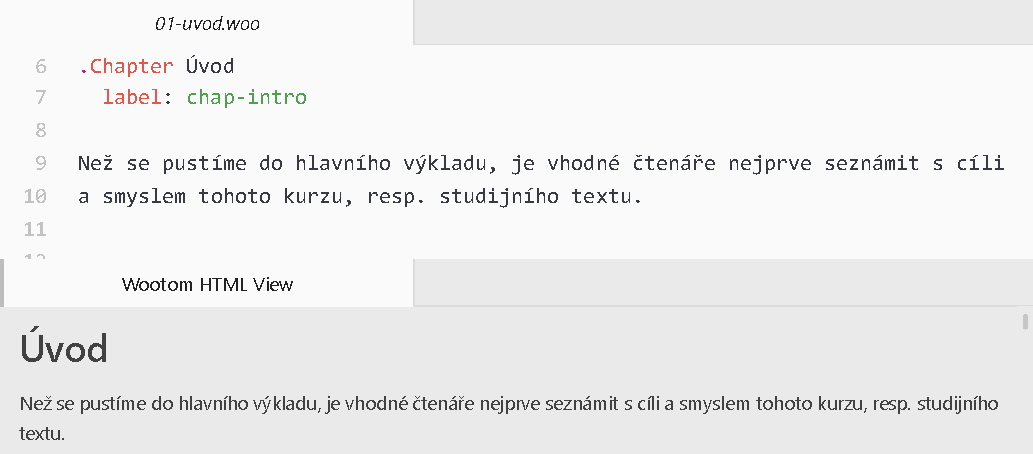
\includegraphics[width=1.0\textwidth]{content/realizace/zobrazení-náhledu-pkm-kapitola}
 	\caption[Náhled části dokumentu]{Náhled části dokumentu ve zdroji studijního textu k BI-PKM~\cite{pkm}}
    \label{zobrazeni-nahledu-pkm-kapitola}
\end{figure}

\begin{sloppypar}
Náhled je živě aktualizován při modifikaci zdrojového souboru. Bylo implementováno jednoduché zobrazování většiny prvků
FIT Template šablony dle stylů existujících výstupů. Zobrazování některých prvků ale zatím podporováno není. Z časových
důvodů nebylo implementováno zobrazení vnějších prostředí \mintinline{text}{.enumerate} a \mintinline{text}{.itemize}
a vnitřního prostředí \mintinline{text}{.item}. Dále nebylo implementováno zobrazování vnějšího prostředí \mintinline
{text}{.image} a vnitřního prostředí \mintinline{text}{.todo}, a to z důvodu jejich absence ve zdrojích existujících
studijních textů. Všechny ostatní prvky jsou (alespoň částečně) zobrazovány.
\end{sloppypar}

Tímto je realizován funkční požadavek \textbf{\ref{F2}} a \textbf{\ref{F3}}. V budoucnu by mohl být náhled vylepšen
například o zobrazení celého dokumentu (nikoliv pouze aktuálně otevřeného souboru) nebo o synchronní posuv náhledu a
zdrojového souboru (což by mělo být možné díky přesným pozicím vrcholů AST).

\subsection{Zobrazování matematických výrazů}

Zobrazování matematických výrazů je na základě provedené rešerše \ref{zobrazovani-matematickych-vyrazu} řešeno za pomoci
knihovny MathJax 2.x s konfigurací SVG výstupu. Uživateli je dále umožněno nadefinovat v nastaveních rozšíření vlastní
makra, která jsou předána konfiguraci knihovny MathJax.

Na obrázku \ref{zobrazeni-nahledu-pkm-matematika} je pro ukázku zobrazen náhled vnitřních matematických prostředí v textu,
jež jsou doplněna o vnější matematické prostředí (blokovou matematiku).

\begin{figure}\centering
    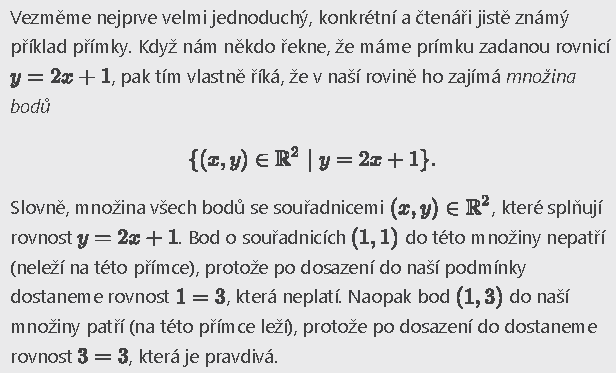
\includegraphics[width=1.0\textwidth]{content/realizace/zobrazení-náhledu-pkm-matematika}
 	\caption[Matematické výrazy v náhledu dokumentu]{Matematické výrazy v náhledu studijního textu k BI-PKM~\cite{pkm}}
    \label{zobrazeni-nahledu-pkm-matematika}
\end{figure}

Protože je sazba matematických výrazů výpočetně náročná, jsou výstupní SVG jsou cachována v paměti (do zavření editoru)
a je-li stejný výraz použit znovu (při obnovení náhledu nebo třeba v jiném souboru), MathJax už volán není a výsledné
SVG je zobrazeno mnohem rychleji (zdánlivě okamžitě).

Byl tak realizován funkční požadavek \textbf{\ref{F4}}.

\subsection{Zobrazování grafických objektů}

Zobrazování TikZ obrázků je na základě provedené rešerše \ref{zobrazovani-grafickych-objektu} řešeno závislostí na
nativní instalaci \TeX{} distribuce. Obdobně jako uživatel může v nastaveních nadefinovat vlastní makra pro MathJax, tak
i zde je umožněno do preambule \LaTeX{} dokumentu, který je použit pro vygenerování obrázku, vložit vlastní obsah (nejen
vlastní makra, ale například i použití dalších \LaTeX{} \textit{packages}).

Při překladu vrcholu AST, který reprezentuje vnější prostředí \mintinline{text}{!tikz}, je nejprve zobrazeno HTML se
(částečně skrytým) zdrojem TikZ. Při tomto překladu je zároveň zavolána asynchronní funkce, která nejprve zkontroluje,
zdali se zdroj obrázku nenachází v cache. Pokud ano, je vrácen obsah cache (kterým je výsledné SVG) a ten je zobrazen
uživateli. Pokud ne, je TikZ zdroj spolu s preambulí (výchozí, nebo uživatelem definovanou) zapsán do dočasného souboru,
na který je zavolán příkaz \mintinline{text}{latex}, jehož výsledkem je DVI soubor (jehož generování je rychlejší, než
PDF). Pro vygenerování SVG z DVI je pak využit příkaz \mintinline{text}{dvisvgm}. Nakonec je SVG výstup přečten, přidán
do cache, jsou uklizeny dočasné soubory a obrázek je zobrazen uživateli. Pokud při procesu nastala chyba, je uživateli
zobrazen namísto obrázku obsah \LaTeX{} logu (log soubor je pak také odstraněn). Cache funguje stejným způsobem jako
cache pro MathJax výstup (je pouze v paměti, po zavření editoru je ztracena).

Protože vygenerované SVG má fixní barvy výplně, je pro podporu různých témat uživatelského rozhraní uživateli umožněno
vybrat v nastaveních jeden ze tří režimů zobrazování těchto SVG výstupů. Výchozím režimem je zobrazení obrázků s bílým
pozadím, dalším režimem pak inverze barev SVG a posledním režimem je zobrazení SVG bez jakýchkoliv změn (není přidáno
pozadí ani pozměněny barvy).

Tímto byl realizován funkční požadavek \textbf{\ref{F5}}. Ukázka náhledu TikZ obrázku se nachází na obrázku \ref
{zobrazeni-nahledu-pkm-tikz}.

\begin{figure}\centering
    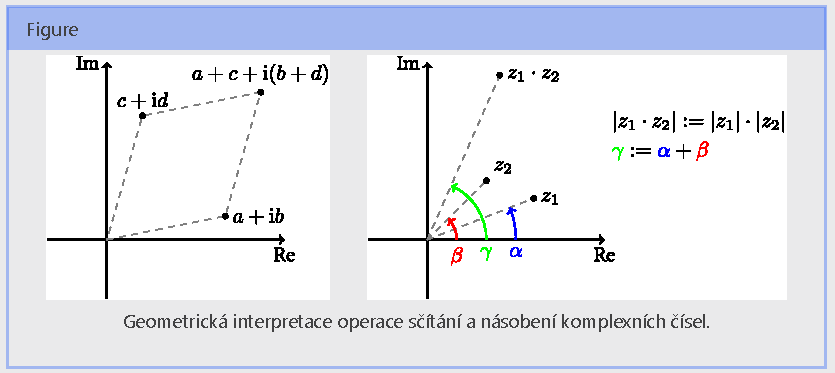
\includegraphics[width=1.0\textwidth]{content/realizace/zobrazení-náhledu-pkm-tikz}
 	\caption[TikZ obrázky v náhledu dokumentu]{TikZ obrázky v náhledu studijního textu k BI-PKM~\cite{pkm}}
    \label{zobrazeni-nahledu-pkm-tikz}
\end{figure}


\section{Navigace}
Navigace v dokumentu je realizována v podobě navigačního podokna, které si uživatel může v pracovním prostředí Atomu
zobrazit s pomocí příkazu \mintinline{text}{wootom:toggleNavigation}, klávesové zkratky (ve výchozím nastavení \textit
{Alt + N}), položky \uv{Wootom: Toggle Navigation} v kontextovém menu nebo podpoložky \uv{Toggle Navigation} položky
\uv{Wootom} v hlavním menu Atomu.

\begin{sloppypar}
Po zobrazení navigačního podokna (které se nejprve zobrazí napravo podokna editoru aktuálně otevřeného souboru; uživatel
si jej případně může přemístit) je aktuálně otevřený soubor rozparsován do AST. Z AST je pak získán seznam všech vrcholů,
které reprezentují části dokumentu a seznam všech vrcholů, které mají v meta-datech neprázdnou položku \mintinline{text}
{label}.
\end{sloppypar}

Ze seznamu vrcholů částí dokumentu je pak vytvořena jednoduchá stromová struktura reflektující úrovně konkrétních částí
(toto je potřeba provést, protože vytvořený AST části nevnořuje podle úrovně) z té je vytvořen číslovaný víceúrovňový
HTML seznam obsahující nadpisy daných částí. Nadpisy jsou přeloženy do HTML s pomocí volání \mintinline{text}
{RenderingManager#render}, čímž je zajištěno i zobrazení případných vnitřních prostředí. Seznam vrcholů AST se značkou
je abecedně seřazen a poté je z něj vytvořen jednoduchý nečíslovaný HTML seznam, obsahující název značky, druh vrcholu
(případě také jeho variantu) a jeho počáteční řádek. Všem položkám obou HTML seznamů je přidán \textit{event listener}
pro událost \textit{click}, který při kliknutí na položku seznamu skočí v editoru aktuálně otevřeného souboru na pozici
začátku daného prvku.

Tyto HTML seznamy jsou vloženy do navigačního podokna a pro přehlednost uvedeny nadpisy. Mezi nadpis a seznam je pak
vždy vloženo textové pole, s jehož pomocí může uživatel v seznamu vyhledávat relevantní položky. Vyhledávání je spuštěno
při libovolném uživatelském vstupu; pokud uživatel svůj dotaz vymaže, je vyhledávání zrušeno. Při vyhledávání v seznamu
částí dokumentu je vyhledáváno v textech nadpisů částí a výsledný seznam je zploštěn (už není víceúrovňový). Při
vyhledávání v seznamu značek je vyhledáváno pouze v názvech značek. Seznam výsledků vyhledávání je seřazen od největší
shody po nejnižší shodu.

Pro vyhledávání byla využita knihovna Fuse.js, která umožňuje fuzzy vyhledávání, kdy dotaz uživatele nemusí přesně
odpovídat vyhledávanému textu (dle dokumentace \cite{fuse-docs} knihovna využívá modifikovanou verzi algoritmu Bitap).
Tato knihovna byla dále vybrána díky její přehledné dokumentaci, dostupnosti TypeScript \textit{types}, permisivní
open-source licenci a velké popularitě (mezi 1,5 miliony a 3 miliony týdenních stažení z npm \cite{npm} za poslední
rok). Knihovna dále dle \cite{fuse-docs} umožňuje upravit mnoho různých parametrů vyhledávání, takže je v případném
budoucím vývoji možno například upravit mezi, které musí shoda dotazu a vyhledávaného textu dosáhnout.

Na obrázku \ref{navigace-pkm} je pro ilustraci zobrazeno okno Atomu s otevřeným souborem zdroje studijního textu k
BI-PKM na levé straně a jeho navigačním podoknem na pravé straně.

\begin{figure}\centering
    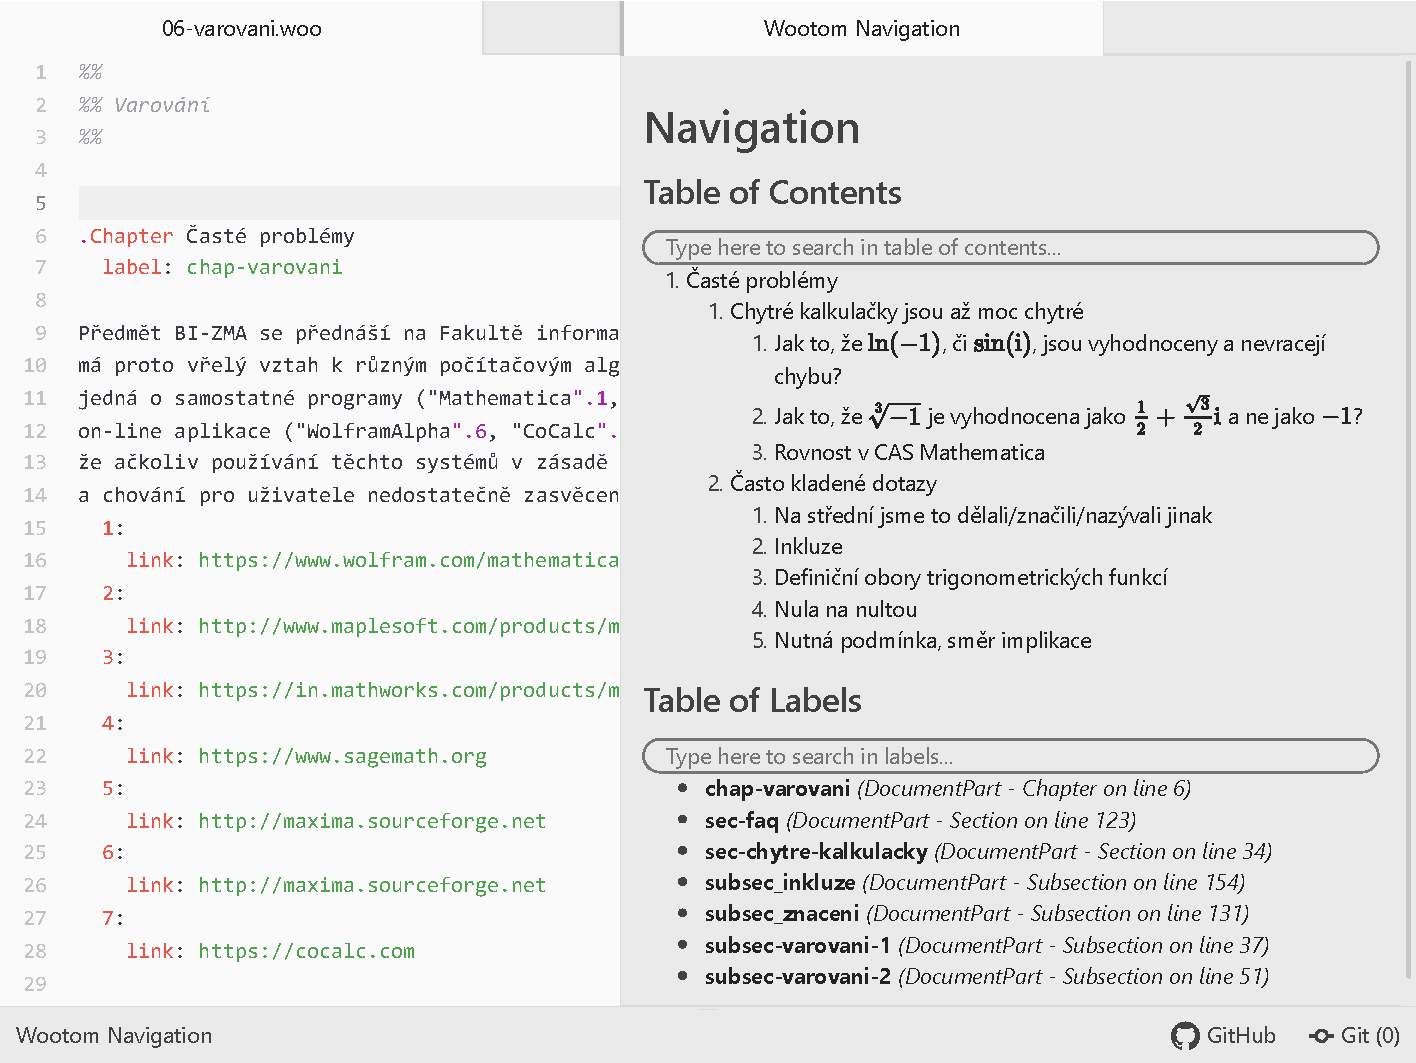
\includegraphics[width=1.0\textwidth]{content/realizace/navigace-pkm}
 	\caption[Navigace v dokumentu]{Navigační podokno u otevřeného souboru zdroje studijního textu k BI-PKM \cite{pkm}}
    \label{navigace-pkm}
\end{figure}

Tímto byly realizovány funkční požadavky \textbf{F6} až \textbf{F10}. Implementaci by bylo dále možno vylepšit například
o zobrazení přehledu částí a značek v celém dokumentu (nikoliv v pouze aktuálně otevřeném souboru).


\section{Testování}
Atom poskytuje v sobě zabudovaný systém pro spouštění testů, takzvaný test runner, postavený na testovacím frameworku
Jasmine. Všechny testy musí být ve složce \mintinline{text}{spec} v kořenové složce package a musí mít ve jméně příponu
\mintinline{text}{-spec} (tedy například \mintinline{text}{main-spec.js}). Následně je všechny testy možno spustit z
terminálu příkazem \mintinline{shell}{atom --test spec} (případně lze namísto celé složky s testy použít seznam
konkrétních souborů s testy), nebo přímo z Atomu s pomocí příkazu \mintinline{text}{window:run-package-specs}, za
předpokladu, že je jako aktuální projekt otevřen testovaný package. \cite{atom-man-specs}

Tento Atomem poskytovaný test runner nicméně vnitřně využívá Jasmine ve verzi 1.3. \cite{atom-man-specs} Jedná se o
poněkud starší verzi z roku 2013. \cite{jasmine-old-release} Chceme-li použít novější verzi Jasmine, nebo dokonce úplně
jiný testovací framework, můžeme využít možnosti vytvoření vlastního test runner. Takto vytvořené test runners pak jde
navíc jednoduše poskytnout ostatním pro využití v jejich packages, které si test runner pouze stáhnou jako závislost z
npm a v \mintinline{text}{package.json} řeknou Atomu, že chtějí využít onen konkrétní test runner. \cite{atom-man-specs}

\#todo Výběr konkrétního test runneru



\begin{conclusion}
	Cílem této práce bylo seznámit se s nově vzniklým formátem WooWoo, prozkoumat možnosti moderních editorů či vývojových
prostředí, zejména co se týče jejich rozšiřitelnosti a navrhnout, implementovat a otestovat rozšíření vybraného editoru,
jehož účelem má být právě poskytnutí chybějící okamžité zpětné vazby při tvorbě WooWoo dokumentů a tím zjednodušení
práce s nimi. Zejména jde pak o přehlednou prezentaci logické struktury dokumentů, zobrazování matematických výrazů a
různých grafických objektů (TikZ diagramy), navigaci mezi různými částmi dokumentu a vyhledávání pomocí značek objektů,
a to s využitím stylů založených na existujících šablonách.

Na základě provedené rešerše bylo vytvořeno rozšíření editoru Atom, protože poskytuje ze zkoumaných editorů největší
prostor pro modifikaci a zároveň poskytuje kvalitní dokumentaci a širokou komunitu pro řešení případných problémů.

Toto rozšíření aktuálně nabízí živý náhled otevřeného kusu dokumentu, který přesně a přehledně prezentuje jeho logickou
strukturu. Náhled také zobrazuje v dokumentu obsažené matematické výrazy s využitím knihovny MathJax 2.6, která
poskytuje dostatečnou podporu LaTeX maker využitých v existujících studijních materiálech psaných s pomocí WooWoo.
Náhled dále zobrazuje TikZ diagramy s využitím nativní TeX distribuce. Rozšíření poskytuje okno s přehledem částí a
značek v otevřeném kusu dokumentu a fuzzy vyhledávání v jejich názvech. Bylo využito stylů založených na existujících
šablonách.

Funkčnost rozšíření byla řádně otestována s využitím unit testů, integračních testů a jednoduchého uživatelského
testování. Dále byly prozkoumány možnosti rozšíření editoru pro podporu více šablon a návrh a implementace probíhaly
tak, aby toto případné další rozšíření šlo provést jen s drobnými modifikacemi.

Vzniklé rozšíření usnadní tvorbu studijních textů ve formátu WooWoo díky poskytnutí okamžité zpětné vazby a nabízí navíc
mnoho možností pro další budoucí rozšíření, jako je podpora zobrazení celého dokumentu (ne jen otevřeného kusu),
synchronní posuv náhledu, lišta nástrojů, podpora více šablon a potenciální vznik celého ekosystému šablonových
rozšíření. Zde implementovaný parser by se navíc mohl potencionálně využít i ve zcela jiných projektech, a to i díky
použité permisivní open source licenci a kódu dostupnému na portálu GitHub.

\end{conclusion}

\printbibliography

\appendix

\chapter{Seznam použitých zkratek}
% \printglossaries
\begin{description}
	\item[AST] Abstraktní syntaktický strom (z anglického abstract syntax tree)
\item[BI-PKM] Přípravný kurz matematiky
\item[BI-ZMA] Základy matematické analýzy
\item[CSS] Cascading Style Sheets
\item[EPUB] Electronic Publication
\item[HTML] Hypertext Markup Language
\item[npm] Node Package Manager
\item[PDF] Portable Document Format
\item[YAML] YAML Ain't Markup Language

\end{description}


% % % % % % % % % % % % % % % % % % % % % % % % % % % % 
% % Tuto kapitolu z výsledné práce ODSTRAŇTE.
% % % % % % % % % % % % % % % % % % % % % % % % % % % % 
% 
% \chapter{Návod k~použití této šablony}
% 
% Tento dokument slouží jako základ pro napsání závěrečné práce na Fakultě informačních technologií ČVUT v~Praze.
% 
% \section{Výběr základu}
% 
% Vyberte si šablonu podle druhu práce (bakalářská, diplomová), jazyka (čeština, angličtina) a kódování (ASCII, \mbox{UTF-8}, \mbox{ISO-8859-2} neboli latin2 a nebo \mbox{Windows-1250}). 
% 
% V~české variantě naleznete šablony v~souborech pojmenovaných ve formátu práce\_kódování.tex. Typ může být:
% \begin{description}
% 	\item[BP] bakalářská práce,
% 	\item[DP] diplomová (magisterská) práce.
% \end{description}
% Kódování, ve kterém chcete psát, může být:
% \begin{description}
% 	\item[UTF-8] kódování Unicode,
% 	\item[ISO-8859-2] latin2,
% 	\item[Windows-1250] znaková sada 1250 Windows.
% \end{description}
% V~případě nejistoty ohledně kódování doporučujeme následující postup:
% \begin{enumerate}
% 	\item Otevřete šablony pro kódování UTF-8 v~editoru prostého textu, který chcete pro psaní práce použít -- pokud můžete texty s~diakritikou normálně přečíst, použijte tuto šablonu.
% 	\item V~opačném případě postupujte dále podle toho, jaký operační systém používáte:
% 	\begin{itemize}
% 		\item v~případě Windows použijte šablonu pro kódování \mbox{Windows-1250},
% 		\item jinak zkuste použít šablonu pro kódování \mbox{ISO-8859-2}.
% 	\end{itemize}
% \end{enumerate}
% 
% 
% V~anglické variantě jsou šablony pojmenované podle typu práce, možnosti jsou:
% \begin{description}
% 	\item[bachelors] bakalářská práce,
% 	\item[masters] diplomová (magisterská) práce.
% \end{description}
% 
% \section{Použití šablony}
% 
% Šablona je určena pro zpracování systémem \LaTeXe{}. Text je možné psát v~textovém editoru jako prostý text, lze však také využít specializovaný editor pro \LaTeX{}, např. Kile.
% 
% Pro získání tisknutelného výstupu z~takto vytvořeného souboru použijte příkaz \verb|pdflatex|, kterému předáte cestu k~souboru jako parametr. Vhodný editor pro \LaTeX{} toto udělá za Vás. \verb|pdfcslatex| ani \verb|cslatex| \emph{nebudou} s~těmito šablonami fungovat.
% 
% Více informací o~použití systému \LaTeX{} najdete např. v~\cite{wikilatex}.
% 
% \subsection{Typografie}
% 
% Při psaní dodržujte typografické konvence zvoleného jazyka. České \uv{uvozovky} zapisujte použitím příkazu \verb|\uv|, kterému v~parametru předáte text, jenž má být v~uvozovkách. Anglické otevírací uvozovky se v~\LaTeX{}u zadávají jako dva zpětné apostrofy, uzavírací uvozovky jako dva apostrofy. Často chybně uváděný symbol "{} (palce) nemá s~uvozovkami nic společného.
% 
% Dále je třeba zabránit zalomení řádky mezi některými slovy, v~češtině např. za jednopísmennými předložkami a spojkami (vyjma \uv{a}). To docílíte vložením pružné nezalomitelné mezery -- znakem \texttt{\textasciitilde}. V~tomto případě to není třeba dělat ručně, lze použít program \verb|vlna|.
% 
% Více o~typografii viz \cite{kobltypo}.
% 
% \subsection{Obrázky}
% 
% Pro umožnění vkládání obrázků je vhodné použít balíček \verb|graphicx|, samotné vložení se provede příkazem \verb|\includegraphics|. Takto je možné vkládat obrázky ve formátu PDF, PNG a JPEG jestliže používáte pdf\LaTeX{} nebo ve formátu EPS jestliže používáte \LaTeX{}. Doporučujeme preferovat vektorové obrázky před rastrovými (vyjma fotografií).
% 
% \subsubsection{Získání vhodného formátu}
% 
% Pro získání vektorových formátů PDF nebo EPS z~jiných lze použít některý z~vektorových grafických editorů. Pro převod rastrového obrázku na vektorový lze použít rasterizaci, kterou mnohé editory zvládají (např. Inkscape). Pro konverze lze použít též nástroje pro dávkové zpracování běžně dodávané s~\LaTeX{}em, např. \verb|epstopdf|.
% 
% \subsubsection{Plovoucí prostředí}
% 
% Příkazem \verb|\includegraphics| lze obrázky vkládat přímo, doporučujeme však použít plovoucí prostředí, konkrétně \verb|figure|. Například obrázek \ref{fig:float} byl vložen tímto způsobem. Vůbec přitom nevadí, když je obrázek umístěn jinde, než bylo původně zamýšleno -- je tomu tak hlavně kvůli dodržení typografických konvencí. Namísto vynucování konkrétní pozice obrázku doporučujeme používat odkazování z~textu (dvojice příkazů \verb|\label| a \verb|\ref|).
% 
% \begin{figure}\centering
% 	
\includegraphics[width=0.5\textwidth, angle=30]{cvut-logo-bw}
% 	\caption[Příklad obrázku]{Ukázkový obrázek v~plovoucím prostředí}\label{fig:float}
% \end{figure}
% 
% \subsubsection{Verze obrázků}
% 
% % Gnuplot BW i barevně
% Může se hodit mít více verzí stejného obrázku, např. pro barevný či černobílý tisk a nebo pro prezentaci. S~pomocí některých nástrojů na generování grafiky je to snadné.
% 
% Máte-li například graf vytvořený v programu Gnuplot, můžete jeho černobílou variantu (viz obr. \ref{fig:gnuplot-bw}) vytvořit parametrem \verb|monochrome dashed| příkazu \verb|set term|. Barevnou variantu (viz obr. \ref{fig:gnuplot-col}) vhodnou na prezentace lze vytvořit parametrem \verb|colour solid|.
% 
% \begin{figure}\centering
% 	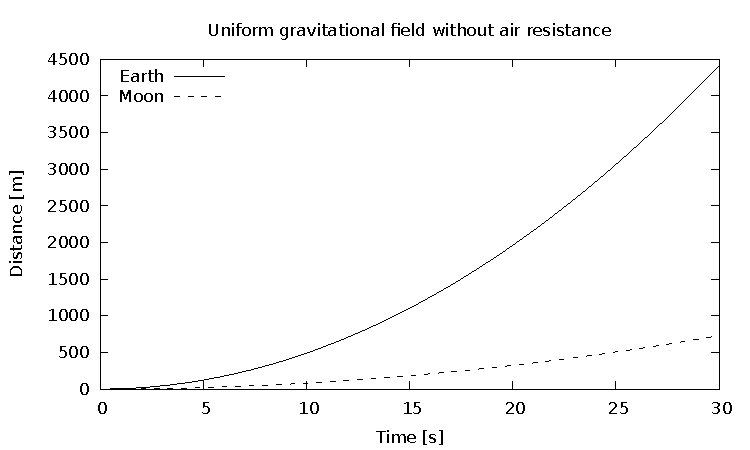
\includegraphics{gnuplot-bw}
% 	\caption{Černobílá varianta obrázku generovaného programem Gnuplot}\label{fig:gnuplot-bw}
% \end{figure}
% 
% \begin{figure}\centering
% 	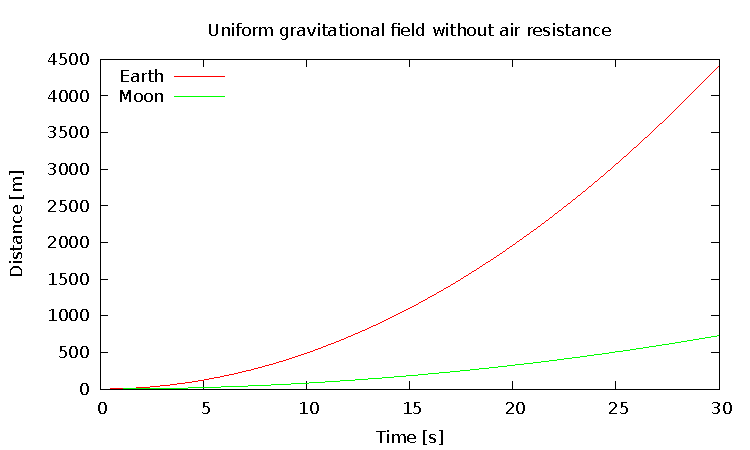
\includegraphics{gnuplot-col}
% 	\caption{Barevná varianta obrázku generovaného programem Gnuplot}\label{fig:gnuplot-col}
% \end{figure}
% 
% 
% \subsection{Tabulky}
% 
% Tabulky lze zadávat různě, např. v~prostředí \verb|tabular|, avšak pro jejich vkládání platí to samé, co pro obrázky -- použijte plovoucí prostředí, v~tomto případě \verb|table|. Například tabulka \ref{tab:matematika} byla vložena tímto způsobem.
% 
% \begin{table}\centering
% 	\caption[Příklad tabulky]{Zadávání matematiky}\label{tab:matematika}
% 	\begin{tabular}{|l|l|c|c|}\hline
% 		Typ		& Prostředí		& \LaTeX{}ovská zkratka	& \TeX{}ovská zkratka	\tabularnewline \hline \hline
% 		Text		& \verb|math|		& \verb|\(...\)|	& \verb|$...$|		\tabularnewline \hline
% 		Displayed	& \verb|displaymath|	& \verb|\[...\]|	& \verb|$$...$$|	\tabularnewline \hline
% 	\end{tabular}
% \end{table}
% 
% % % % % % % % % % % % % % % % % % % % % % % % % % % % 

\chapter{Obsah přiloženého CD}

%upravte podle skutecnosti

\begin{figure}
	\dirtree{%
		.1 readme.txt\DTcomment{stručný popis obsahu CD}.
		.1 exe\DTcomment{adresář se spustitelnou formou implementace}.
		.1 src.
		.2 impl\DTcomment{zdrojové kódy implementace}.
		.2 thesis\DTcomment{zdrojová forma práce ve formátu \LaTeX{}}.
		.1 text\DTcomment{text práce}.
		.2 thesis.pdf\DTcomment{text práce ve formátu PDF}.
		.2 thesis.ps\DTcomment{text práce ve formátu PS}.
	}
\end{figure}

\end{document}
